%% ******************************************************
%% * This work may be distributed and/or modified under *
%% * the conditions of the LaTeX Project Public License *
%% *     http://www.latex-project.org/lppl.txt          *
%% * either version 1.3c of this license or any later   *
%% * version.                                           *
%% ******************************************************
\PassOptionsToPackage{quiet}{xeCJK}
\PassOptionsToPackage{quiet}{fontspec}
\PassOptionsToPackage{no-math}{fontspec}
\documentclass[11pt]{article}
\usepackage{geometry}
\usepackage{indentfirst,setspace}
\usepackage[toc]{multitoc}
\setlength{\parindent}{2em}
\setstretch{1.25}
\usepackage{pdfpages}
\usepackage[level]{datetime}
\usepackage{unicode-math,xeCJK}
\usepackage{authblk}
\setmainfont{Libertinus Serif}
\setsansfont{Libertinus Sans}
\setCJKmainfont{SimSong}[BoldFont=Chiron Sung HK, ItalicFont=Kaiti SC]
\makeatletter
\usepackage{listings,dirtree}
\lstdefinestyle{TeX}{
    language      =  [LaTeX]TeX,
    texcsstyle    =  *\color{H7},
    numbers       =  none,
    basicstyle    =  {\small\color{H6}\tt},
    mathescape    =  false,
    breaklines    =  true,
    columns       =  fixed,
    keywordstyle  =  \color{H3},
    commentstyle  =  \color{darkgray},
    tabsize       =  2,
    keywords      =  {mail,flyleaf,sticker,logo,notebook,chapter,newnote,newnotesss,newnotessss,emptynote,newhdunote,
    makeframe,course,more}
}
\usepackage{hyperref,xcolor,verbatim}

\definecolor{pkgcolor}{Hsb}{103,.8,.5}
\definecolor{moducolor}{Hsb}{290,.8,.5}
\definecolor{cmdcolor}{Hsb}{188,.8,.5}
\definecolor{filecolor}{Hsb}{207,.6,.7}
\definecolor{H1}{Hsb}{349,.8,.8}% 海棠紅 (Hangzhou MTR L 1 )
\definecolor{H2}{Hsb}{23, .8,.8}% 丹桂橙 (Hangzhou Metro 2 )
\definecolor{H3}{Hsb}{48, .8,.8}% 柠檬黄 (Hangzhou Metro 3 )
\definecolor{H4}{Hsb}{103,.8,.8}% 香樟绿 (Hangzhou Metro 4 )
\definecolor{H5}{Hsb}{188,.8,.8}% 青藍色 (Hangzhou MTR L 5 )
\definecolor{H6}{Hsb}{207,.8,.8}% 海洋蓝 (Hangzhou Metro 6 )
\definecolor{H7}{Hsb}{290,.8,.8}% 浪漫紫 (Hangzhou Metro 7 )
\hypersetup{colorlinks,urlcolor=H1,linkcolor=H2,filecolor=filecolor,pdfstartview=FitH,pdfview=FitH,pdfcreator=XeTeX output}

\renewcommand*\l@subsection{\@dottedtocline{2}{1.5em}{2.1em}}
\def\pkg#1{\texorpdfstring{\textcolor{pkgcolor}{\textsf{#1}}}{“#1”}}
\def\mode#1{\texorpdfstring{\textcolor{moducolor}{\textsf{#1}}}{“#1”}}
\def\cmd#1{\texorpdfstring{\textcolor{cmdcolor}{\textsf{#1}}}{“#1”}}
\def\datechange#1#2{%
  \noindent{\makebox[\textwidth][r]{\color{H7}\rule{1.15\textwidth}{.4pt}}}
  \noindent\makebox[0pt][r]{\makebox[-3em][r]{\small\textbf{\textcolor{H7}{#1}}}\;\;}{\sffamily Update: \ignorespaces#2}}
\makeatother

\title{The \pkg{LiteTable} Template}
\author[1]{Xia Mingyu, \href{https://www.hdu.edu.cn}{Hangzhou Dianzi University}}
\yyyymmdddate
\date{\today}
\affil[1]{\href{mailto:xiamyphys@gmail.com}{\texttt{xiamyphys@gmail.com}}}
\date{\today\quad Version 2.2a\thanks{%
  \url{https://github.com/xiamyphys/litetable}}}
\begin{document}
\maketitle

\vspace{-2em}
\begin{abstract}
\pkg{LiteTable} 模板提供了一个多彩的课程表设计,本文档为\pkg{LiteTable} 模板的说明文档.

\end{abstract}

\tableofcontents\clearpage

\section{Introduction}

\subsection{本模板的目的}
本模板提供了一个多彩的课程表设计. 

如果你在使用本模板时遇到问题,或者有更好的建议,或者你想参与本模板或本人其他模板的开发,欢迎通过邮件 \href{mailto:xiamyphys@gmail.com}{xiamyphys@gmail.com} 联络我.

同样,你也可以加入我的\textsf\LaTeX{} 技術交流群 \href{https://qm.qq.com/q/OnHzbNvVAG}{QQ Group: 760570712} 与我交流,来获取模板的内测版本.

\subsection{所需宏集}
本模板基于 \pkg{standalone} 文档类开发. 其需要 \pkg{tikz} 宏集去绘制图形,\pkg{kvoptions} 和 \pkg{etoolbox} 宏集用于提供全局选项,\pkg{expl3} 宏基用于支持数组,\pkg{ctex}宏集用于支持中文语言,\pkg{fontawesome5} 宏集提供一系列精美的图标.

我强烈建议您使用终端机去执行以下命令,以将所有宏集更新到最新版本
\begin{verbatim}
    tlmgr update --self
    tlmgr update --all
\end{verbatim}

如果您所在的地区存在网路封锁,你可以选择合适的镜像网站或其他方法\footnote{请遵循当地的网路条例.}. 欲详细了解,请前往 \href{https://tex.stackexchange.com/questions/55437/how-do-i-update-my-tex-distribution}{How do I update my TEX distribution?}

\subsection{载入 \pkg{LiteTable} 和其模式}
将文件 \verb|litetable.cls| 保存至你的项目根目录,然后创立一个 \verb|.tex| 文件,只需在第一行输入命令 \verb|\documentclass{litetable}| 即可.

本模板提供了三个模式:\mode{date},\mode{style} 和 \mode{font}. 只需将你想要使用的模式选项分别添加在你的 \verb|.tex| 文件中命令 \verb|\documentclass[options]{litetable}| 的方括号中即可.

\newpage
\section{\pkg{LiteTable} 的模式}
\begin{verbatim}
  \documentclass[options]{litetable}
\end{verbatim}
\subsection{\mode{date} 模式}
此模式有两个选项,\mode{en} 和 \mode{cn},可分别使工作日以英文或大陆简体显示,默认为英文.

\subsection{\mode{style} 模式}
此模式有两个选项,\mode{round} 和 \mode{sharp},可分别使课程块圆角或直角显示,默认为直角.

\subsection{\mode{font} 模式}
此模式有两个选项,\mode{times} 和 \mode{libertinus},可分别使字体为 ``Times New Roman'' 或 ``Libertinus'',默认为 ``Times New Roman''.\footnote{在使用 ``Libertinus'' 选项前请确保电脑中已安装该字体.}

\section{\pkg{LiteTable} 的命令}

\subsection{\cmd{makeframe} 命令}
\begin{verbatim}
    \makeframe{Timetable -- Semester 5}
\end{verbatim}

此命令可建立一个标题为 ``Timetable -- Semester 5'' 的空白课程表.

\subsection{The \cmd{timelist} command}
\begin{verbatim}
    \timelist{
      8:05,8:55,10:00,10:50,11:40,13:30,14:20,15:15,16:05,18:30,19:20,20:10;
      8:50,9:40,10:45,11:35,12:25,14:15,15:05,16:00,16:50,19:15,20:05,20:55
    }
\end{verbatim}

此命令可将时间添加至课程表的左侧,内容的第一行是每节课程开始时间,第二行是每节课程的结束时间,时间之间用逗号(\verb|,|)分隔,第一行与第二行之间用分号(\verb|;|)分隔.

本课程表目前只支持每天12节课. 在后续更新中,将支持自定义每天的课程节数,敬请期待!

\subsection{\cmd{course} 命令}
\begin{verbatim}
    \course{H5}{3}{5}{AQM}{Building 6·225}{Yuan Li \& Mengnan Chen}{Week 1 -- 18}
\end{verbatim}

此命令共有7个变量.
\begin{itemize}
  \item 第一个为你想选择的课程块颜色,从 ``H1'' 到 ``H9'' 可选.
  \item 第二个和第三个为课程的起始节数和结束节数.
  \item 第四个为课程的名称.
  \item 第五个为课程的地址.
  \item 第六个为教师的名字.
  \item 第七个为课程的起始周和结束周.
\end{itemize}

\subsection{\cmd{newday} 命令}
此命令可切换当前日到第二天,此时课程块会右移一格.

\subsection{\cmd{more} 命令}
\begin{verbatim}
  \more{·School Start: 04 / 03 / 2024 ·Summer Vacation: 05 / 07 / 2024}
\end{verbatim}
此命令可在课程表末尾添加备注信息.

\subsection{\cmd{sticker} 命令}
\begin{verbatim}
  \sticker{favicon}
\end{verbatim}
在使用此命令后页面的右下方会添加一张贴纸.

\newpage
\section{版本历史}

课程表的设计源于杭电助手(\href{https://www.hdu.edu.cn}{杭州电子科技大学}\footnote{https://en.wikipedia.org/wiki/Hangzhou\_Dianzi\_University})学生课表页面\footnote{仅本校师生可访问.} 页面排版十分精美,于是本人使用\LaTeX{} 复刻出了课程表样式,并制作成模板分享给大家.

\textsf{\bfseries Version 1.0} 于01/09/2023完成开发,并发布在\href{https://www.latexstudio.net/index/details/index/mid/3625.html}{LaTeX 工作室} (杭州萧山)和\href{http://xhslink.com/od7Ycw}{小红书}上,赢得了许多人的喜爱.

\textsf{\bfseries Version 2.0a}于01/11/2023完成开发,并发布在\href{https://www.latexstudio.net/index/details/index/mid/3636.html}{LaTeX 工作室} (杭州萧山)和\href{http://xhslink.com/od7Ycw}{小红书}上. 此版本使用 \verb|.cls| 文件,使 \verb|main.tex| 文件更简洁. 同时,此版本添加了全局选项,可设置 ``课程块" 显示为圆角或直角. 此版本也支持一个 \verb|.tex| 文件中生成多张课表.

\textsf{\bfseries Version 2.1a} 于05/11/2023完成开发. 支持 libertinus 字体.

\textsf{\bfseries Version 2.2a} 于31/01/2024完成开发. 此版本修复了分辨率超出的bug,更改纸张类型为美国信纸并支持自定义课程起始和结束时间.

\datechange{01/09/2023}{Version 2.0a}
\begin{itemize}
    \item 支持课程块显示为圆角或直角.
    \item 支持一个 \verb|.tex| 文件中生成多张课表.
\end{itemize}

\datechange{05/11/2023}{Version 2.1a}
\begin{itemize}
    \item 支持 libertinus 字体.
\end{itemize}

\datechange{31/01/2024}{Version 2.2a}
\begin{itemize}
    \item 修复了分辨率超出的bug.
    \item 更改纸张类型为美国信纸.
    \item 支持自定义课程起始和结束时间.
    \item 支持在页面右下角添加一个你喜欢的小贴纸.
\end{itemize}

\newpage\setstretch{1}
\appendix
\section{代码示例}
\lstinputlisting[style=TeX]{litetable-demo.tex}

\includepdf[pages=last-1,nup=1x2,angle=90]{litetable-demo.pdf}
\end{document}